% 第 4 章下半部分：命题 4、推论 1、命题 5、命题 6 与更新过程仿真中的恒等式
% label 前缀 pb-

\subsection{命题 4：预算约束下的期数与规模}

\subsubsection{原式与参数含义}

命题 4 回答的问题是在总监测规模固定时，预算应当分给更多的观测期，还是分给更大的单期规模。原文第 237 行设定了一个理想化的重复采样设计。设计者在 $T$ 个观测期内设定相同的每期真实风险集规模 $n_T=B/(\rho T)$，记设计方案为 $\mathcal D_T=(T,n_T)$，并假定 $\bar R$、$\rho$、$k$、$v_R$ 不随期变化。给定完整环境扰动序列后，各期的分支传播与报告抽样相互条件独立。跨期基础水平 $\bar R$ 的估计量取各期矩估计量的样本平均，原文的定义如下式所示：
\begin{equation*}
\overline{\widehat{R}}_T \triangleq \frac{1}{T} \sum_{t=1}^T \widehat{R}_t = \frac{1}{T} \sum_{t=1}^T \frac{C_t}{\rho n_T}.
\tag{原文式 14}
\end{equation*}

命题 4（原文第 244–263 行）共有三条结论。第 (i) 条在环境扰动跨期独立时给出平均估计量的精确方差，如下式所示：
\begin{equation*}
\operatorname{Var}(\overline{\widehat{R}}_T \mid n_T) = \frac{v_R}{T} + \frac{A}{B},
\tag{原文式 15}
\end{equation*}
第 (ii) 条在环境扰动服从一阶自回归时给出有效独立期数形式的近似，如下式所示：
\begin{equation*}
\operatorname{Var}(\overline{\widehat{R}}_T \mid n_T) \approx \frac{v_R}{T_{\operatorname{eff}}(T, r)} + \frac{A}{B}, \qquad T_{\operatorname{eff}}(T, r) \triangleq T \frac{1-r}{1+r},
\tag{原文式 16}
\end{equation*}
第 (iii) 条给出严格用尽预算且各期风险集为相同正整数时可供比较的期数集合，如下式所示：
\begin{equation*}
\mathcal{T}(B, \rho) \triangleq \left\{ T \in \mathbb{N}_+ \;:\; \frac{B}{\rho T} \in \mathbb{N}_+ \right\}.
\tag{原文式 17}
\end{equation*}

附录对第 (ii) 条给出了有限期数下的精确双重求和闭式，它是本节推导的核心，原文写法如下：
\begin{equation*}
\operatorname{Var}\left(\sum_{t=1}^T R_t \;\middle|\; n_T\right) = T v_R + 2 v_R \sum_{s=1}^{T-1} (T-s) r^s = v_R T \left[\frac{1+r}{1-r} - \frac{2r(1-r^T)}{T(1-r)^2}\right].
\tag*{原文第 751 行}
\end{equation*}

各式中出现的参数含义如下。
\begin{itemize}
\item $T$ 是观测期数，取正整数，在命题 4 中是设计者可以选择的变量。
\item $n_T$ 是每期上一代真实风险集人数，只有取正整数时才对应一个可以实施的设计。
\item $\rho\in(0,1]$ 是报告率，即每个真实感染最终被报告的概率。
\item $m=\rho n_T$ 是每期期望被报告规模，单位为例/期，与第~\ref{sec:model} 节定义的 $m$ 相同。
\item $B=Tm$ 是总监测输入规模，即各期期望被报告人数之和，单位为例；它与推论 1 中以货币计的总经费 $\mathcal B$ 是两个不同的量。
\item $C_t$ 是第 $t$ 期的报告病例数，$\widehat R_t=C_t/(\rho n_T)$ 是第 $t$ 期的矩估计量，命题 1 已证明它同时是极大似然估计量且条件无偏。
\item $\bar R>0$ 是跨期基础传播水平，$v_R=\operatorname{Var}(R_t)\ge 0$ 是环境方差，$k>0$ 是个体离散参数。
\item $A=\bar R+\rho(\bar R^2+v_R)/k$ 是命题 2 的方差系数；原文第 251 行特意说明它与估计目标“目标 A”同名而含义不同。
\item $r\in[0,1)$ 是环境扰动的一阶自回归系数，满足 $\operatorname{Cov}(R_t,R_{t+s}\mid n_T)=v_Rr^{|s|}$；它与命题 6 中负二项累积分布函数 $F_{\operatorname{NB}}(x;r,p)$ 的形状参数同名，后者取 $r=nk$，两者无关。
\item $T_{\operatorname{eff}}(T,r)$ 是有效独立期数，$\mathcal T(B,\rho)$ 是可行期数集合，$\mathbb N_+$ 是正整数集合。
\end{itemize}

\subsubsection{逐步推导}

第 (i) 条的推导以整条环境序列 $\{R_t\}$ 为条件，分七步完成。
\begin{enumerate}
\item 由原文第 238 行的设计假定，给定 $\{R_t\}$ 后各期相互条件独立；再由命题 1 的条件无偏性 $\mathbb E[\widehat R_t\mid R_t,n_T]=R_t$，内层条件期望为 $\mathbb E[\overline{\widehat R}_T\mid\{R_t\},n_T]=\frac1T\sum_{t=1}^TR_t$。
\item 以 $\{R_t\}$ 为条件应用全方差公式（附录引理~\ref{lem:ap-totvar}），总方差拆成两项：
\begin{equation*}
\operatorname{Var}(\overline{\widehat R}_T\mid n_T)=\operatorname{Var}\Big(\frac1T\sum_{t=1}^TR_t\;\Big|\;n_T\Big)+\mathbb E\big[\operatorname{Var}(\overline{\widehat R}_T\mid\{R_t\},n_T)\,\big|\,n_T\big].
\end{equation*}
\item 由方差的二次齐次性 $\operatorname{Var}(cY)=c^2\operatorname{Var}(Y)$，第一项等于 $T^{-2}\operatorname{Var}(\sum_tR_t\mid n_T)$。
\item 由条件独立随机变量之和的方差等于各自方差之和，内层条件方差为 $T^{-2}\sum_t\operatorname{Var}(\widehat R_t\mid R_t,n_T)$；代入命题 1 的条件方差（原文式 6）得到每一期的条件方差为 $R_t/(\rho n_T)+R_t^2/(kn_T)$。
\item 对每一期取期望时使用二阶矩关系 $\mathbb E[R_t^2]=\bar R^2+v_R$（原文第 728 行），得 $\bar R/(\rho n_T)+(\bar R^2+v_R)/(kn_T)$；再以 $1/n_T=\rho/m$ 代换，它等于 $\frac1m[\bar R+\rho(\bar R^2+v_R)/k]=A/m$，这一步与命题 2 把原文式 7 改写为 $v_R+A/m$ 的过程完全相同。
\item 把 $T$ 个相同的 $A/m$ 相加再除以 $T^2$，第二项等于 $A/(Tm)$，也就是附录第 743–747 行第三行中的 $A/(T\rho n_T)$；用预算约束 $Tm=B$ 代换后第二项等于 $A/B$，与 $T$ 无关。
\item 环境跨期独立时，独立变量和的方差可加，$\operatorname{Var}(\sum_tR_t)=Tv_R$，第一项等于 $v_R/T$；两项相加即得原文式 15，而对 $T$ 求导得 $-v_R/T^2<0$，所以固定 $B$ 时增加 $T$ 严格降低方差。
\end{enumerate}

第 (ii) 条需要计算相关随机变量之和的方差。附录用错位相减完成这一步，下面给出一条按行求和的路线，每一步都只用到有限等比级数。
\begin{enumerate}
\item 由方差的双线性展开，得到下式：
\begin{equation*}
\operatorname{Var}\Big(\sum_{t=1}^T R_t\Big)=\sum_{t=1}^T\sum_{u=1}^T\operatorname{Cov}(R_t,R_u).
\end{equation*}
再代入一阶自回归过程的自协方差 $\operatorname{Cov}(R_t,R_u)=v_Rr^{|t-u|}$ \citep{hamilton1994time}，所求方差等于一个 $T\times T$ 矩阵全部元素之和。
\item 按间隔 $s=|t-u|$ 分组计数：对角线上 $s=0$ 的元素有 $T$ 个，每个等于 $v_R$；间隔为 $s\ge1$ 的有序对在上三角与下三角各有 $T-s$ 个，共 $2(T-s)$ 个，于是得到附录闭式的第一个等号
\begin{equation}
\operatorname{Var}\Big(\sum_{t=1}^TR_t\Big)=Tv_R+2v_R\sum_{s=1}^{T-1}(T-s)r^s .\label{eq:pb-sumcov}
\end{equation}
\item 式~\eqref{eq:pb-sumcov} 中的级数等于上三角元素（除以 $v_R$）之和；按行计算，第 $t$ 行对角线右侧有 $j=T-t$ 个元素，由有限等比级数公式其和为 $r+r^2+\dots+r^j=r(1-r^j)/(1-r)$，再对 $j=1,\dots,T-1$ 求和并对 $\sum_{j=1}^{T-1}r^j$ 再用一次等比级数公式，得
\begin{equation*}
\sum_{s=1}^{T-1}(T-s)r^s=\sum_{j=1}^{T-1}\frac{r(1-r^j)}{1-r}=\frac{r(T-1)}{1-r}-\frac{r^2(1-r^{T-1})}{(1-r)^2}.
\end{equation*}
\item 通分化简时把 $\frac{r(T-1)}{1-r}$ 拆成 $\frac{rT}{1-r}-\frac{r(1-r)}{(1-r)^2}$，与第二项合并后分子为 $r(1-r)+r^2-r^{T+1}=r(1-r^T)$，于是
\begin{equation*}
\sum_{s=1}^{T-1}(T-s)r^s=\frac{rT}{1-r}-\frac{r(1-r^T)}{(1-r)^2}.
\end{equation*}
\item 代回式~\eqref{eq:pb-sumcov} 并利用恒等式 $1+\frac{2r}{1-r}=\frac{1+r}{1-r}$，得 $Tv_R+\frac{2v_RrT}{1-r}-\frac{2v_Rr(1-r^T)}{(1-r)^2}=v_RT\big[\frac{1+r}{1-r}-\frac{2r(1-r^T)}{T(1-r)^2}\big]$，这就是附录第 751 行的第二个等号。
\item 把闭式除以 $T^2$，得到 AR(1) 环境下平均估计量环境项的精确表达
\begin{equation}
\operatorname{Var}\Big(\frac1T\sum_{t=1}^TR_t\Big)=\frac{v_R}{T}\Big[\frac{1+r}{1-r}-\frac{2r(1-r^T)}{T(1-r)^2}\Big],\label{eq:pb-exactenv}
\end{equation}
总方差等于式~\eqref{eq:pb-exactenv} 加上与 $r$ 无关的 $A/B$，因为第 (i) 条第 4–6 步只用到给定 $\{R_t\}$ 时的条件独立性，与环境序列的相关结构无关。
\item 原文式 16 相当于丢掉方括号中的第二项，此时环境项变为 $\frac{v_R}{T}\cdot\frac{1+r}{1-r}=v_R/T_{\operatorname{eff}}$；由于 $0\le r<1$ 时 $1-r^T>0$，被丢掉的项非负且在 $r>0$ 时严格为正，所以该近似对环境项恒高估，等价于恒低估有效期数。
\item 用近似值除以精确值再减 1，并把分子分母同乘 $T(1-r)^2$，得到相对高估比例的闭式
\begin{equation}
\frac{\text{近似环境项}}{\text{精确环境项}}-1=\frac{2r(1-r^T)}{T(1-r)(1+r)-2r(1-r^T)} .\label{eq:pb-overrate}
\end{equation}
\item 当 $T$ 增大时 $r^T\to0$，且分母中的 $2r(1-r^T)$ 相对 $T(1-r^2)$ 可以忽略，由此得到式~\eqref{eq:pb-overrate} 的一阶近似 $2r/[T(1-r^2)]$；它说明相对误差只以 $1/T$ 的速度衰减，误差的刻度是 $2r/(1-r^2)$ 期，$r=0.8$ 时约为 4.44 期。
\end{enumerate}

第 (iii) 条只涉及整除关系，推导分三步。
\begin{enumerate}
\item 由 $m=\rho n_T$ 与 $B=Tm$ 联立解出 $n_T=B/(\rho T)$，所以 $B/\rho=Tn_T$。
\item 若要求 $n_T\in\mathbb N_+$，则 $B/\rho$ 是正整数 $T$ 与正整数 $n_T$ 的乘积，必须是正整数；因此当 $B/\rho\notin\mathbb N_+$ 时可行集为空，当 $B/\rho\in\mathbb N_+$ 时条件等价于 $T$ 整除 $B/\rho$，可行集就是 $B/\rho$ 的全部正因子。
\item 由于正整数的任何正因子都不超过它本身，$T\le\lfloor B/\rho\rfloor$ 是属于 $\mathcal T(B,\rho)$ 的必要条件，但满足该不等式而不整除 $B/\rho$ 的 $T$ 仍不可行，所以它只是必要条件，充分性不成立。
\end{enumerate}

\subsubsection{直觉与数值例}

总报告数一定时，抽样噪声只取决于报告总数，这是负二项计数在独立相加下方差可加的直接结果，所以 $A/B$ 与切分方式无关；环境噪声则只能靠增加期数来平均。纯人数预算下的最优设计因此是把期数拉到最大，而无限多期在现实中不可行，推论 1 引入每期固定成本 $c_0$ 正是为了修正这一点。

取论文图 1 参数 $\bar R=1.15$、$v_R=0.04$、$k=0.35$、$\rho=0.25$，此时 $A=1.15+0.25\times(1.3225+0.04)/0.35=2.1232$。设总规模 $B=260$ 例，比较两种设计。
\begin{itemize}
\item 设计一为 $T=10$、$m=26$：环境项 $v_R/T=0.004$，抽样项 $A/B=2.1232/260=0.008166$，独立环境下总方差为 $0.01217$。
\item 设计二为 $T=26$、$m=10$：环境项 $0.04/26=0.001538$，抽样项仍为 $0.008166$，总方差为 $0.00970$。两种设计的抽样项完全相同，差别全部来自环境项。
\item 若环境自相关 $r=0.8$，设计一的方括号为 $9-1.6\times(1-0.8^{10})/(10\times0.04)=9-3.5705=5.4295$，由式~\eqref{eq:pb-exactenv} 得精确环境项 $0.004\times5.4295=0.02172$，总方差 $0.02988$；而原文式 16 给出环境项 $0.004\times9=0.036$，总方差 $0.04417$。环境项被高估 65.8\%。
\item 同样在 $r=0.8$ 下，设计二的精确总方差为 $0.01965$，近似值为 $0.02201$。按式~\eqref{eq:pb-overrate}，分子 $1.6\times(1-0.8^{26})=1.5952$，分母 $26\times0.2\times1.8-1.5952=7.7648$，环境项高估 20.5\%；对应的精确有效期数为 3.48，而 $T_{\operatorname{eff}}=26\times0.2/1.8=2.89$。
\end{itemize}

图~\ref{fig:pb-ar1} 给出式~\eqref{eq:pb-overrate} 在 $T=8$ 到 80 上的完整曲线。$r=0.3$ 与 $r=0.5$ 时高估幅度在 $T\ge20$ 后已降到个位数，$r=0.8$ 时曲线下降缓慢，$T=80$ 仍有数个百分点。若要求环境项误差不超过 5\%，在 $r=0.8$ 下按一阶近似约需 $T\approx89$，按精确式需 $T=94$。

\begin{figure}[!tbp]\centering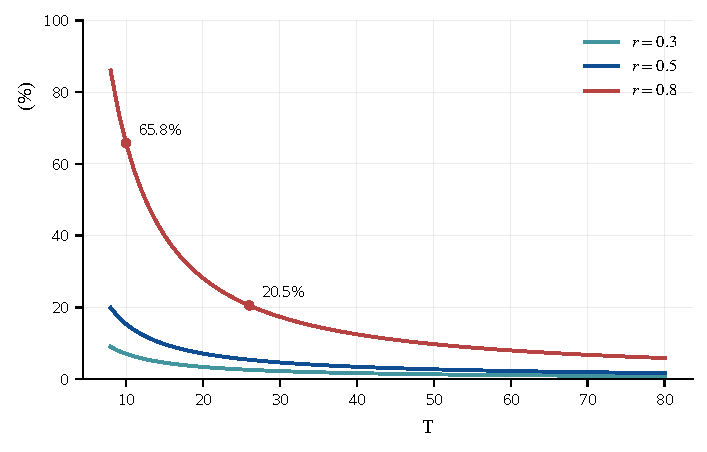
\includegraphics[width=0.62\linewidth]{figures/fig_ar1_teff.pdf}\caption{有效期数近似 $T_{\operatorname{eff}}=T(1-r)/(1+r)$ 对环境方差项的相对高估幅度。横轴为观测期数 $T$，纵轴为近似值相对附录精确闭式的高估百分比，三条曲线对应 $r=0.3$、$0.5$、$0.8$；$r=0.8$ 时 $T=10$ 高估 65.8\%，$T=26$ 仍高估 20.5\%。}\label{fig:pb-ar1}\end{figure}

可行集的三个例子如下。$B=30$、$\rho=0.25$ 时 $B/\rho=120$，可行期数是 120 的 16 个正因子 $\{1,\allowbreak 2,\allowbreak 3,\allowbreak 4,\allowbreak 5,\allowbreak 6,\allowbreak 8,\allowbreak 10,\allowbreak 12,\allowbreak 15,\allowbreak 20,\allowbreak 24,\allowbreak 30,\allowbreak 40,\allowbreak 60,\allowbreak 120\}$；$B=30$、$\rho=0.7$ 时 $B/\rho=42.86$ 带有小数部分，可行集为空；$T=7$ 满足 $7\le120$，但 7 不整除 120，所以不可行。

\subsubsection{与仿真和实证的对应}

论文的图 1–3 都没有直接检验命题 4，正文第 264–269 行只给出机制解释。本讲义的核验分三层完成。
\begin{itemize}
\item 符号核验确认了第 (i) 条的全方差推导与 $\partial/\partial T=-v_R/T^2$，并在 $T=1,\dots,40$ 上逐个确认式~\eqref{eq:pb-sumcov} 的级数与按行求和闭式恒等，附录第 751 行的两个等号均成立。
\item 蒙特卡洛核验在图 1 参数下比较了 $T=10$、$m=26$（20000 次重复）与 $T=26$、$m=10$（7692 次重复）两种设计、$r\in\{0,0.5,0.8\}$ 六种情形。模拟方差与精确闭式全部在 $|z|<3$ 内一致，例如 $T=10$、$r=0.8$ 时模拟值 0.02998 对精确值 0.02988（$z=0.33$），$T=26$、$r=0.8$ 时 0.01895 对 0.01965（$z=-2.31$）；同一情形下原文式 16 的近似值 0.04417 与 0.02201 明显偏离模拟值。
\item 在 $r\in[0,0.98]$、$T\le300$ 的网格上，式~\eqref{eq:pb-exactenv} 关于 $T$ 严格递减，所以命题 4(i) 中“增加 $T$ 严格降低方差”的结论在 AR(1) 环境下仍然成立，这一点论文没有说明。
\end{itemize}
可行集的三个例子（120 的 16 个正因子、空集、$T=7$ 的反例）也逐一得到确认。实证部分（第~\ref{sec:empirical} 节）没有估计周增长比的自相关系数，所以 $r$ 的取值在本文中仍是情景参数。

\subsubsection{原文表述的问题}

\begin{itemize}
\item 第 254–256 行称在 $T\gg1/(1-r)$ 时原文式 16 是“良好近似”，但没有说明近似方向。由第 7 步，近似恒高估环境项，从设计角度看偏保守；$T=26$、$r=0.8$ 时 $T(1-r)=5.2$，已大于 $1/(1-r)=5$，误差仍有 20.5\%。附录第 753 行说丢掉的是 $O(1/T^2)$ 项，这在绝对量上成立，但相对主项只是 $O(1/T)$。建议正文直接写出附录第 751 行的精确闭式（它本身就是初等函数），把 $T_{\operatorname{eff}}$ 作为直觉保留，并写明近似方向。
\item 方差系数 $A$ 与“目标 A”同名，AR(1) 系数 $r$ 与负二项形状参数 $r=nk$ 同名，答辩时容易被追问，建议改记方差系数为 $\kappa$、AR(1) 系数为 $\phi$，或把两类估计目标改称“目标 I”“目标 II”。
\end{itemize}

\subsection{推论 1：成本最优的单期规模}

\subsubsection{原式与参数含义}

推论 1 在命题 4 的基础上引入两类成本：每个观测期的固定运转成本 $c_0>0$，以及每捕获一个报告病例的边际成本 $c_1>0$。原文第 274 行给出的总经费约束如下：
\begin{equation*}
\mathcal{B} = T(c_0 + c_1 m)
\tag*{原文第 274 行}
\end{equation*}
同一行给出的待最小化目标函数如下：
\begin{equation*}
\operatorname{Var}(\overline{\widehat{R}}_T) = \frac{v_R}{T} + \frac{A}{T m}
\tag*{原文第 274 行}
\end{equation*}
推论 1 的结论是唯一内部最优单期规模，原文写法如下：
\begin{equation*}
m^* = \sqrt{\frac{c_0}{c_1} \cdot \frac{A}{v_R}} = \sqrt{\frac{c_0}{c_1} m_\times}.
\tag{原文式 18}
\end{equation*}
若内部解超出可行上界，原文第 279 行给出的角点解如下：
\begin{equation*}
m^* = \frac{\mathcal{B} - c_0}{c_1}
\tag*{原文第 279 行}
\end{equation*}
原文第 280 行在 AR(1) 环境下先把环境方差替换为有效环境方差：
\begin{equation*}
v_{\mathrm{eff}} \approx v_R \frac{1+r}{1-r}
\tag*{原文第 280 行}
\end{equation*}
并由此给出修正后的最优单期规模：
\begin{equation*}
m^*_{\mathrm{AR}} \approx \sqrt{\frac{c_0}{c_1} m_\times \frac{1-r}{1+r}} < m^*
\tag*{原文第 280 行}
\end{equation*}

各式中出现的参数含义如下。
\begin{itemize}
\item $c_0>0$ 是每个观测期的固定成本，例如哨点的运转与维持开销，单位为货币/期。
\item $c_1>0$ 是每个报告病例的边际成本，单位为货币/例；若按覆盖人群计的人均成本为 $c_1'$，覆盖 $n$ 人的花费 $c_1'n=c_1'm/\rho$，所以 $c_1=c_1'/\rho$。
\item $\mathcal B>0$ 是总经费预算；为保证 $T\ge1$，单期规模须满足 $m\le(\mathcal B-c_0)/c_1$。
\item $T\ge1$ 是期数，推论中先按连续变量处理；$m>0$ 是单期期望报告规模。
\item $m_\times=A/v_R$ 是定义 1 的方差占比交叉点，图 1 参数下 $m_\times=53.08$。
\item $v_{\mathrm{eff}}$ 是 AR(1) 环境下的有效环境方差，$m^*_{\mathrm{AR}}$ 是相应的近似最优规模，$r\in[0,1)$ 的含义同命题 4。
\end{itemize}

\subsubsection{逐步推导}

\begin{enumerate}
\item 由预算约束解出 $T=\mathcal B/(c_0+c_1m)$，代入目标函数 $\frac1T(v_R+A/m)$，展开乘积后得到只含 $m$ 的一元函数
\begin{equation}
f(m)=\frac{(c_0+c_1m)(v_R+A/m)}{\mathcal B}=\frac{c_0v_R+c_0A/m+c_1v_Rm+c_1A}{\mathcal B}.\label{eq:pb-fm}
\end{equation}
\item 由幂函数求导法则对式~\eqref{eq:pb-fm} 逐项求导，常数项 $c_0v_R$ 与 $c_1A$ 的导数为零，得 $f'(m)=(c_1v_R-c_0A/m^2)/\mathcal B$。
\item 再求一次导数得 $f''(m)=2c_0A/(\mathcal Bm^3)$，它在 $m>0$ 上恒正，所以 $f$ 在 $(0,\infty)$ 上严格凸，一阶条件的正根若存在就是唯一的全局最小点，这就是原文第 275 行二阶导的含义。
\item 令 $f'(m)=0$ 得 $m^2=c_0A/(c_1v_R)$，取正根，并代入定义 1 的 $m_\times=A/v_R$，即得原文式 18。
\item 把 $m^*$ 代回式~\eqref{eq:pb-fm}，由 $m^{*2}=c_0A/(c_1v_R)$ 可得两个随 $m$ 变化的项相等，$c_0A/m^*=c_1v_Rm^*=\sqrt{c_0c_1Av_R}$；再用完全平方公式合并，最小方差为
\begin{equation}
f(m^*)=\frac{c_0v_R+c_1A+2\sqrt{c_0c_1Av_R}}{\mathcal B}=\frac{\big(\sqrt{c_0v_R}+\sqrt{c_1A}\big)^2}{\mathcal B}.\label{eq:pb-fmin}
\end{equation}
\item 同一结果也可以由算术–几何平均不等式 $c_0A/m+c_1v_Rm\ge2\sqrt{c_0c_1Av_R}$ 直接读出，取等条件 $c_0A/m=c_1v_Rm$ 正是第 4 步的一阶条件。
\item 若把 $T$ 与 $m$ 都当作连续变量并用 Lagrange 乘子法，令 $u=1/T$，在约束 $c_0+c_1m=\mathcal Bu$ 下最小化 $u(v_R+A/m)$，对 $u$ 与 $m$ 的一阶条件分别为 $v_R+A/m=\lambda\mathcal B$ 与 $uA/m^2=\lambda c_1$；消去 $\lambda$ 后得 $c_1(v_R+A/m)=(c_0+c_1m)A/m^2$，即 $c_1v_R=c_0A/m^2$，与代入法一致。
\item 可行性 $T\ge1$ 等价于 $m\le(\mathcal B-c_0)/c_1$；由于凸函数 $f$ 在 $m^*$ 左侧单调递减，当 $m^*$ 超出这一上界时，可行域内的最小点落在上界本身，对应 $T=1$，这就是原文第 279 行的角点解。
\item 当 $c_0=0$ 时 $f'(m)=c_1v_R/\mathcal B>0$，$f$ 单调递增，最优 $m\to0$，回到命题 4 中纯人数预算下“期数越多越好”的结论。
\item 在 AR(1) 环境下，由原文式 16 有 $v_R/T_{\operatorname{eff}}=v_{\mathrm{eff}}/T$，目标函数的形式不变，只是 $v_R$ 换成 $v_{\mathrm{eff}}=v_R(1+r)/(1-r)$；重复第 1–4 步得 $m^*_{\mathrm{AR}}=\sqrt{c_0A/(c_1v_{\mathrm{eff}})}=\sqrt{(c_0/c_1)m_\times(1-r)/(1+r)}$，由于 $r>0$ 时 $(1-r)/(1+r)<1$，有 $m^*_{\mathrm{AR}}<m^*$。
\item 期数 $T$ 在实际中必须是整数；对每个整数 $T$ 取用尽预算的 $m=(\mathcal B/T-c_0)/c_1$，计算 $(v_R+A/m)/T$ 并逐一比较，即得整数约束下的最优设计，连续解 $m^*$ 只是这一枚举的下界参照。
\end{enumerate}

推论 1 与经典两阶段抽样的费用分配在数学上同构 \citep{cochran1977sampling}。Cochran 第 10 章讨论等大小初级单元的二阶抽样：抽取 $n$ 个初级单元、每个单元内抽取 $m$ 个次级单元，无限总体下估计量方差为 $S_b^2/n+S_w^2/(nm)$，总成本为 $\kappa_1n+\kappa_2nm$，最优次级样本量为 $m_{\rm opt}=\sqrt{(\kappa_1/\kappa_2)(S_w^2/S_b^2)}$。表~\ref{tab:pb-cochran} 给出逐项对应，把右列代入即得原文式 18。Cochran 在有限总体下 $S_b^2$ 的位置是 $S_1^2-S_2^2/M$，本文环境层相当于无限总体，这一位置就是 $v_R$。

\begin{table}[!tbp]\centering\small\caption{推论 1 与 Cochran 两阶段抽样的符号对应}\label{tab:pb-cochran}
\begin{tabular}{L{3.6cm}L{4.2cm}L{4.2cm}}
\toprule
Cochran 符号 & Cochran 中的含义 & 推论 1 中的对应 \\
\midrule
$n$ & 初级单元数 & 期数 $T$ \\
$m$ & 每个初级单元内的次级单元数 & 单期期望报告规模 $m$ \\
$S_b^2$ & 初级单元间方差 & 环境方差 $v_R$ \\
$S_w^2$ & 初级单元内方差 & 方差系数 $A$ \\
$\kappa_1$ & 每个初级单元的成本 & 每期固定成本 $c_0$ \\
$\kappa_2$ & 每个次级单元的成本 & 每例边际成本 $c_1$ \\
$S_w^2/S_b^2$ & 单元内外方差比 & 交叉点 $m_\times=A/v_R$ \\
\bottomrule
\end{tabular}
\end{table}

\subsubsection{直觉与数值例}

$c_0$ 是多开一期的代价，$c_1$ 是多数一个病例的代价。原文式 18 说明 $m^*$ 是成本比 $c_0/c_1$ 与统计平衡点 $m_\times$ 的几何平均：固定成本越高，每期越应多收病例；环境越稳定（$v_R$ 越小、$m_\times$ 越大），越值得在单期内做大规模。

在图 1 参数下 $m_\times=53.08$。$c_0/c_1=10$ 时 $m^*=\sqrt{10\times53.08}=23.0$，$c_0/c_1=100$ 时 $m^*=\sqrt{100\times53.08}=72.9$。图~\ref{fig:pb-budget} 左图画出目标函数 $(c_0/c_1+m)(v_R+A/m)$ 相对其最小值的倍数，两条曲线在 $m^*$ 附近都很平坦，单期规模偏离最优值一倍以内时方差的损失有限，偏离一个数量级时损失迅速增大。

原文第 283 行给出的 $m^*\approx14.6\sim22.2$ 与 $46.1\sim70.2$ 取自第 515 行流感住院情景的交叉点区间 $m_\times\in[21.3,49.3]$，与图 1 参数无关，具体换算如下：$\sqrt{10\times21.3}=14.59$，$\sqrt{10\times49.3}=22.20$，$\sqrt{100\times21.3}=46.15$，$\sqrt{100\times49.3}=70.21$。该情景取 $\bar R\approx1.67$、$k\in[0.2,0.5]$、$\rho\in[0.0056,0.021]$、$v_R\in[0.04,0.08]$。$m_\times=\bar R/v_R+\rho(\bar R^2+v_R)/(kv_R)$ 在 $v_R=0.04$、$\rho=0.021$、$k=0.2$ 的角点取最大值，此时 $A=1.67+0.021\times(2.7889+0.04)/0.2=1.96703$，$m_\times=49.18$；论文的 49.3 相当于在 $A$ 中取 $v_R=0.08$、分母取 $0.04$，两处 $v_R$ 不一致。按一致参数修正后，上端为 $\sqrt{10\times49.18}=22.18$ 与 $\sqrt{100\times49.18}=70.13$，差异很小，但口径应当统一。下端角点 $v_R=0.08$、$\rho=0.0056$、$k=0.5$ 给出 $m_\times=21.28$，与论文一致。

连续松弛与整数解在小预算下可能相差很大。取 $c_0=100$、$c_1=1$、$\mathcal B=600$ 与图 1 参数，连续解 $m^*=72.86$，对应 $T=600/(100+72.86)=3.47$，由式~\eqref{eq:pb-fmin} 得连续松弛下界 $(\sqrt{100\times0.04}+\sqrt{2.1232})^2/600=(2+1.4571)^2/600=0.01992$。表~\ref{tab:pb-enum} 列出 $T=1,\dots,5$ 的整数枚举，整数最优为 $T=3$、$m=100$，与连续解 72.86 相差 37\%，方差 0.02041 比连续下界高约 2.5\%。图~\ref{fig:pb-budget} 右图把同一枚举画成柱图。预算较大时两者几乎重合：$c_0=100$、$\mathcal B=2\times10^4$ 时连续解 72.86（$T=115.70$），整数最优 $T=116$、$m=72.41$；$c_0=10$、$\mathcal B=2000$ 时连续解 23.04，整数最优 $T=61$、$m=22.79$。

\begin{table}[!tbp]\centering\small\caption{整数期数枚举（$c_0=100$，$c_1=1$，$\mathcal B=600$，图 1 参数）}\label{tab:pb-enum}
\begin{tabular}{L{2.4cm}L{3.6cm}L{4.6cm}}
\toprule
期数 $T$ & 单期规模 $m=\mathcal B/T-c_0$ & 跨期估计量方差 $(v_R+A/m)/T$ \\
\midrule
1 & 500 & 0.04425 \\
2 & 200 & 0.02531 \\
3 & 100 & 0.02041 \\
4 & 50 & 0.02062 \\
5 & 20 & 0.02923 \\
连续松弛 & 72.86（$T=3.47$） & 0.01992 \\
\bottomrule
\end{tabular}
\end{table}

\begin{figure}[!tbp]\centering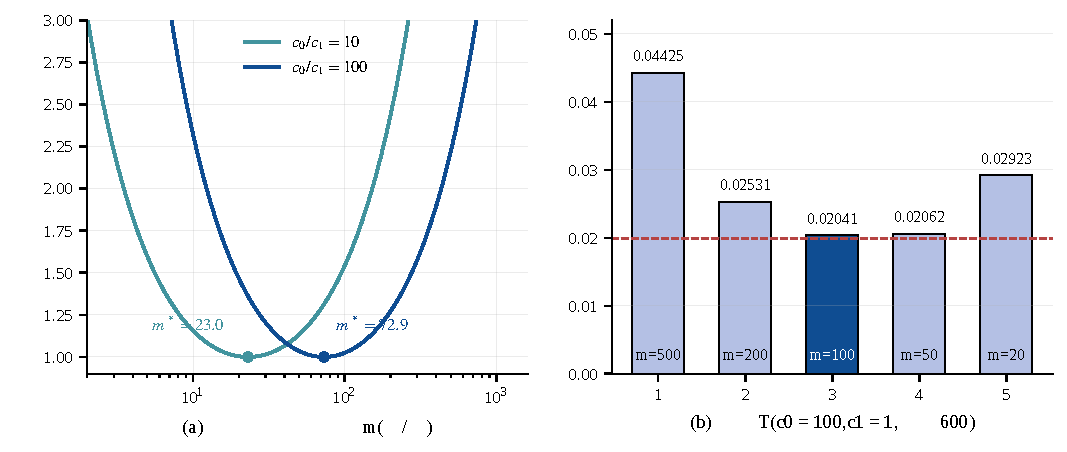
\includegraphics[width=0.95\linewidth]{figures/fig_budget.pdf}\caption{推论 1 的连续最优与整数枚举（图 1 参数）。左图横轴为单期期望报告规模 $m$（对数刻度），纵轴为目标函数 $(c_0/c_1+m)(v_R+A/m)$ 相对其最小值的倍数，$c_0/c_1=10$ 与 $100$ 两条曲线分别在 $m^*=23.0$ 与 $72.9$ 处取最小值；右图为 $c_0=100$、$c_1=1$、预算 600 时 $T=1,\dots,5$ 的跨期估计量方差，$T=3$（$m=100$）最小，红虚线为连续松弛下界。}\label{fig:pb-budget}\end{figure}

AR(1) 修正的方向与命题 4 一致。$c_0/c_1=100$、$r=0.5$ 时 $(1-r)/(1+r)=1/3$，$m^*_{\mathrm{AR}}=\sqrt{100\times53.08/3}=42.1$；$r=0.8$ 时该因子为 $1/9$，$m^*_{\mathrm{AR}}=72.86/3=24.3$。改用式~\eqref{eq:pb-exactenv} 的精确环境项、在 $\mathcal B=2\times10^4$ 下做整数搜索，最优单期规模分别为 42.9（$T=140$）与 25.0（$T=160$）。近似式高估环境项，因而略微低估最优单期规模。

\subsubsection{与仿真和实证的对应}

论文没有为推论 1 设计仿真，图 1–3 也不涉及成本。本讲义的核验覆盖了全部代数步骤：代入后的目标函数、一阶与二阶导数、唯一正根、几何平均形式、$c_0=0$ 时的单调性以及 AR(1) 替换后的 $m^*_{\mathrm{AR}}$ 均经符号核验成立；角点情形 $c_0=100$、$c_1=1$、$\mathcal B=140$ 时内部解 72.9 超过上界 40，最优取 $m^*=40$、$T=1$，与原文第 279 行一致。数值方面，第 283 行的两个区间可由第 515 行情景的 $m_\times$ 区间完全复现；图 1 参数下的 23.0 与 72.9、表~\ref{tab:pb-enum} 的整数枚举以及 AR(1) 下的 42.9 与 25.0 均为直接计算结果。实证部分估计的经验交叉点 $m_\times^{\rm emp}=22.6$ 若代入原文式 18，可得 $c_0/c_1=10$ 时的 $m^*$ 参照，但第~\ref{sec:empirical} 节指出经验 $a$、$b$ 都被放大，这一代入只能作为数量级参考。

\subsubsection{原文表述的问题}

\begin{itemize}
\item 第 283 行的数值区间紧接图 1 参数的上下文，却用了第 515 行情景的 $m_\times$，来源没有写明；建议改写为“以第 515 行流感情景的 $m_\times\in[21.3,49.2]$ 为例”，并同步修正第 515 行的 49.3。中期报告把该区间写成“14.6～24.4”，材料中不存在 24.4，属误引。
\item 推论按连续 $T$ 求解，小预算下整数最优可以与连续解相差 37\%；建议补一句“$T$ 须为整数，预算较小时应枚举”。
\item 第 283 行只说与两阶段抽样同构，建议给出表~\ref{tab:pb-cochran} 那样的符号对应与 Cochran 的章节号，答辩时可以直接引用。
\item 第 280 行的 $m^*_{\mathrm{AR}}$ 继承了原文式 16 的高估方向，与精确整数搜索相差约 2\%–3\%，建议注明近似方向，或直接用精确闭式搜索。
\end{itemize}

\subsection{命题 5：仅报告可见时的单步预测方差}

\subsubsection{原式与参数含义}

命题 5 处理时间序列情形：真实感染历史不可见，预测只能依据截至第 $t$ 期的报告历史 $\mathcal F_t^C$。原文先用更新过程描述下一期的感染压力，如下式所示：
\begin{equation*}
\Lambda_{t+1} = \sum_{s=1}^S w_s I_{t+1-s}, \qquad \sum_{s=1}^S w_s = 1.
\tag{原文式 19}
\end{equation*}
原文随后假定给定感染压力与当期传播参数时，下一期真实感染的条件均值为二者之积，如下式所示：
\begin{equation*}
\mathbb{E}[I_{t+1} \mid \Lambda_{t+1}, R_{t+1}, \mathcal{F}_t^C] = \Lambda_{t+1} R_{t+1}.
\tag{原文式 20}
\end{equation*}
报告环节沿用二项抽稀，并假定给定 $I_{t+1}$ 后报告与既往报告历史条件独立，原文第 297 行的写法如下：
\begin{equation*}
C_{t+1} \mid I_{t+1} \sim \operatorname{Binomial}(I_{t+1}, \rho)
\tag*{原文第 297 行}
\end{equation*}
命题 5（原文第 299–308 行）的第一式给出真实感染的预测方差分解：
\begin{equation*}
\operatorname{Var}(I_{t+1} \mid \mathcal{F}_t^C) = \operatorname{Var}\big(\Lambda_{t+1} R_{t+1} \;\big|\; \mathcal{F}_t^C\big) + \mathbb{E}\Big[\operatorname{Var}\big(I_{t+1} \;\big|\; \Lambda_{t+1}, R_{t+1}, \mathcal{F}_t^C\big) \;\Big|\; \mathcal{F}_t^C\Big].
\tag{原文式 21}
\end{equation*}
第二式给出报告病例的预测方差分解：
\begin{equation*}
\operatorname{Var}(C_{t+1} \mid \mathcal{F}_t^C) = \rho(1 - \rho)\,\mathbb{E}[I_{t+1} \mid \mathcal{F}_t^C] + \rho^2 \operatorname{Var}(I_{t+1} \mid \mathcal{F}_t^C).
\tag{原文式 22}
\end{equation*}

各式中出现的参数含义如下。
\begin{itemize}
\item $I_{t+1}$ 是第 $t+1$ 期的真实新发感染数，取非负整数，不可观测。
\item $\Lambda_{t+1}$ 是下一期的感染压力，即过去 $S$ 期真实感染按世代间隔权重 $w_s\ge0$ 的加权和；由于它由不可见的 $I$ 构成，给定 $\mathcal F_t^C$ 时它仍是随机变量。
\item $S$ 是世代间隔的最大滞后期数，$w_s$ 满足 $\sum_sw_s=1$。
\item $R_{t+1}$ 是第 $t+1$ 期的传播参数，含义同第~\ref{sec:model} 节。
\item $\mathcal F_t^C$ 是由报告序列 $C_1,\dots,C_t$ 生成的信息集，代表预测时刻能看到的全部数据。
\item $C_{t+1}$ 是第 $t+1$ 期的报告病例数，$\rho\in(0,1]$ 是报告率。
\end{itemize}

\subsubsection{逐步推导}

两式都由条件形式的全方差公式（附录引理~\ref{lem:ap-totvar}）得到，区别在于条件变量的选择。
\begin{enumerate}
\item 记更大的信息集 $\mathcal H=\sigma(\Lambda_{t+1},R_{t+1},\mathcal F_t^C)\supseteq\mathcal F_t^C$，由嵌套信息集下的全方差公式 $\operatorname{Var}(Y\mid\mathcal F)=\operatorname{Var}(\mathbb E[Y\mid\mathcal H]\mid\mathcal F)+\mathbb E[\operatorname{Var}(Y\mid\mathcal H)\mid\mathcal F]$，取 $Y=I_{t+1}$ 即得两项之和。
\item 把原文式 20 的条件均值 $\mathbb E[I_{t+1}\mid\mathcal H]=\Lambda_{t+1}R_{t+1}$ 代入第一项，即得原文式 21；第一项刻画感染压力与传播参数在报告信息下的不确定性，第二项刻画给定二者后的分支抽样噪声。
\item 第二式改以 $I_{t+1}$ 为条件，由全方差公式得到附录给出的展开：
\begin{equation*}
\operatorname{Var}(C_{t+1} \mid \mathcal{F}_t^C) = \mathbb{E}[\operatorname{Var}(C_{t+1} \mid I_{t+1}, \mathcal{F}_t^C) \mid \mathcal{F}_t^C] + \operatorname{Var}(\mathbb{E}[C_{t+1} \mid I_{t+1}, \mathcal{F}_t^C] \mid \mathcal{F}_t^C).
\tag*{原文第 769 行}
\end{equation*}
\item 由二项分布的均值 $np$ 与方差 $np(1-p)$，并利用报告与历史条件独立的假定（原文第 297 行），得 $\mathbb E[C_{t+1}\mid I_{t+1},\mathcal F_t^C]=\rho I_{t+1}$ 与 $\operatorname{Var}(C_{t+1}\mid I_{t+1},\mathcal F_t^C)=\rho(1-\rho)I_{t+1}$（原文第 771 行）。
\item 外层第一项由条件期望的线性性得 $\rho(1-\rho)\mathbb E[I_{t+1}\mid\mathcal F_t^C]$，外层第二项由方差的二次齐次性得 $\rho^2\operatorname{Var}(I_{t+1}\mid\mathcal F_t^C)$，两者相加即得原文式 22。
\end{enumerate}

上述推导除原文式 20 与二项报告外没有用到任何分布假定，所以命题 5 的两式是恒等式，本身不含可以计算的量。为了看清“单代公式不能直接外推”的具体含义，下面在两个附加假定下把它展开。第一个假定是：给定 $\mathcal F$（下文省略下标 $t$ 与 $t+1$），$I\mid\Lambda,R\sim\mathrm{NB}\big(k\Lambda,\,k/(k+R)\big)$，即 $\Lambda$ 个有效感染者各自按第~\ref{sec:model} 节的负二项分支产生后代（附录引理~\ref{lem:ap-nb}）。第二个假定是 $\Lambda$ 与 $R$ 在 $\mathcal F$ 下条件独立，$\mathbb E[R\mid\mathcal F]=\bar R$，$\operatorname{Var}(R\mid\mathcal F)=v_R$。记 $E_\Lambda$、$V_\Lambda$ 为 $\Lambda$ 的条件均值与条件方差，$\mathrm{CV}^2(\Lambda\mid\mathcal F)=V_\Lambda/E_\Lambda^2$。
\begin{enumerate}
\item 由负二项分布 $\mathrm{NB}(r,p)$ 的均值 $r(1-p)/p$ 与方差 $r(1-p)/p^2$，取 $r=k\Lambda$、$p=k/(k+R)$，有 $(1-p)/p=R/k$，所以条件均值为 $\Lambda R$（与原文式 20 相符），条件方差为 $\Lambda R(k+R)/k=\Lambda R+\Lambda R^2/k$。
\item 由独立随机变量乘积的二阶矩 $\mathbb E[\Lambda^2R^2]=\mathbb E[\Lambda^2]\mathbb E[R^2]$ 与 $\mathbb E[Y^2]=\operatorname{Var}(Y)+(\mathbb EY)^2$，原文式 21 的第一项为
\begin{equation*}
\operatorname{Var}(\Lambda R\mid\mathcal F)=(V_\Lambda+E_\Lambda^2)(v_R+\bar R^2)-E_\Lambda^2\bar R^2=V_\Lambda v_R+V_\Lambda\bar R^2+E_\Lambda^2v_R .
\end{equation*}
\item 由条件独立下期望的乘积性质，原文式 21 的第二项为 $\mathbb E[\Lambda R+\Lambda R^2/k\mid\mathcal F]=E_\Lambda\bar R+E_\Lambda(\bar R^2+v_R)/k$；同理 $\mathbb E[I\mid\mathcal F]=E_\Lambda\bar R$。
\item 把第 2、3 步代入原文式 22，并用 $\rho(1-\rho)E_\Lambda\bar R+\rho^2E_\Lambda\bar R=\rho E_\Lambda\bar R$ 合并两个一次项，得
\begin{equation*}
\operatorname{Var}(C\mid\mathcal F)=\rho E_\Lambda\bar R+\frac{\rho^2E_\Lambda(\bar R^2+v_R)}{k}+\rho^2E_\Lambda^2v_R+\rho^2V_\Lambda(\bar R^2+v_R).
\end{equation*}
\item 记 $m\triangleq\rho E_\Lambda$（下一期的期望报告规模在 $R$ 取 1 时的刻度），两边除以 $m^2$；前两项分别化为 $\bar R/m$ 与 $\rho(\bar R^2+v_R)/(km)$，合起来正是 $A/m$，于是
\begin{equation}
\frac{\operatorname{Var}(C\mid\mathcal F)}{(\rho E_\Lambda)^2}=v_R+\frac{A}{m}+\mathrm{CV}^2(\Lambda\mid\mathcal F)\,(\bar R^2+v_R).\label{eq:pb-expand}
\end{equation}
\end{enumerate}
式~\eqref{eq:pb-expand} 的左端是统计量 $C/(\rho E_\Lambda)$ 的条件方差，这个统计量在感染压力已知时就是命题 2 中的单期估计量。当 $\Lambda$ 在 $\mathcal F$ 下已知时 $\mathrm{CV}^2=0$，式~\eqref{eq:pb-expand} 恰好退化为命题 2 的 $v_R+A/m$；真实感染不可见带来的额外项是 $\mathrm{CV}^2(\Lambda\mid\mathcal F)(\bar R^2+v_R)$，它不随 $m$ 以 $1/m$ 衰减，大小取决于从报告历史反推感染压力的精度。

\subsubsection{直觉与数值例}

原文式 22 的两项分别对应两层随机性：给定真实感染后报告环节的二项噪声，以及真实感染本身的预测不确定性经 $\rho^2$ 缩放后的贡献。式~\eqref{eq:pb-expand} 进一步把后者拆成三块，其中前两块与单代模型相同，第三块是“看不见感染”这一事实本身的代价。

取图 1 参数 $\bar R=1.15$、$v_R=0.04$、$k=0.35$、$\rho=0.25$（$A=2.1232$），并设 $E_\Lambda=40$，则 $m=\rho E_\Lambda=10$。
\begin{itemize}
\item 感染压力已知（$\mathrm{CV}=0$）时，式~\eqref{eq:pb-expand} 右端为 $0.04+2.1232/10=0.25232$，乘以 $m^2=100$ 得 $\operatorname{Var}(C\mid\mathcal F)=25.23$；真实感染的预测方差为 $40\times1.15+40\times1.3625/0.35+40^2\times0.04=46+155.71+64=265.71$。
\item 感染压力的条件变异系数为 $\mathrm{CV}=0.3$ 时，额外项为 $0.09\times1.3625=0.12263$，右端变为 $0.37495$，$\operatorname{Var}(C\mid\mathcal F)=37.49$，比感染压力已知时高 48.6\%；真实感染的预测方差增加 $V_\Lambda(\bar R^2+v_R)=144\times1.3625=196.2$，变为 461.9。
\item 设 $E_\Lambda=200$、$\mathrm{CV}=0.5$，则 $m=50$，右端为 $0.04+0.04246+0.25\times1.3625=0.42309$，$\operatorname{Var}(C\mid\mathcal F)=0.42309\times2500=1057.72$。此时额外项 0.3406 远大于规模项 0.0425，继续扩大单期规模几乎无法降低预测方差。
\end{itemize}

\subsubsection{与仿真和实证的对应}

蒙特卡洛核验在上述三种配置下检验了原文式 21、式 22 与式~\eqref{eq:pb-expand}。真实感染方差的模拟值 266.1、456.6、16065.4 与理论值 265.7、461.9、16233.6 的偏离都在 $|z|<3$ 内；报告病例方差在 $\mathrm{CV}=0$ 时模拟值 25.24 对理论 25.23，$E_\Lambda=200$、$\mathrm{CV}=0.5$ 时 1048.12 对 1057.72（$z=-1.76$）。$E_\Lambda=40$、$\mathrm{CV}=0.3$ 的报告病例方差单次模拟为 36.97，对理论 37.49 的 $z=-4.45$；用 20 组独立随机数流各 $10^4$ 次重复复核后，相对误差为 $-0.07\%\pm0.27\%$，与零无差异，所以这是重尾分布下单次模拟的波动，与公式无关。感染压力固定时，$\operatorname{Var}(C)/(\rho\Lambda)^2$ 的模拟值 0.2524 与命题 2 的 0.2523 一致，验证了退化关系。

论文本身没有为命题 5 单独设计仿真。式~\eqref{eq:pb-expand} 的额外项为图 3 的更新过程仿真提供了解释框架：在更新过程中感染压力由报告历史近似，额外项不随规模衰减，这与本节后文式 28 中的偏差项方向一致。第~\ref{sec:empirical} 节实证截距 $a$ 高于情景隐含 $v_R/\bar R^2$ 的现象，也需要这类额外项参与解释。

\subsubsection{原文表述的问题}

\begin{itemize}
\item 命题 5 的两式是对任意分布都成立的全方差恒等式，命题本身没有用到负二项结构，也没有给出可计算的结论。第 309 行称它表明“单代静态公式不能直接外推”，但这一含义要在式~\eqref{eq:pb-expand} 的展开中才看得见；建议把该展开作为命题 5 的推论写进正文。
\item 第 312 行“瓶颈属于目标 B；作为对照，目标 A 在单期不存在瓶颈……”与上下文没有衔接，其中的“目标 A”又与方差系数 $A$ 同名；建议删除，或改写为式~\eqref{eq:pb-expand} 额外项的解释。
\item 附录第 756 行标题“命题 5 的数学证明”实际证明的是正文命题 6（增长检验），第 761 行标题“命题 6 的数学证明”实际证明的是正文命题 5（预测方差分解）。正文第 310、336 行的交叉引用指向正确的 label，错误只在标题文字；建议交换两个小节的标题，答辩材料一律按正文编号。
\end{itemize}

\subsection{命题 6：精确增长检验与功效}

\subsubsection{原式与参数含义}

命题 6 利用命题 1 的精确负二项条件分布，检验当期传播是否超临界。原文的单侧假设如下式所示：
\begin{equation*}
H_0: R_t \le 1 \qquad \text{对} \qquad H_1: R_t > 1.
\tag{原文式 23}
\end{equation*}
命题 6(i) 规定离散临界值取使边界点超额拒绝概率受控的最小整数：
\begin{equation*}
c_\alpha = \min \left\{ c \in \mathbb{N} \;:\; \Pr_{R_t = 1}(C_t \ge c) \le \alpha \right\};
\tag{原文式 24}
\end{equation*}
命题 6(ii) 给出备择 $R_t=1+\delta$ 下的精确功效：
\begin{equation*}
\pi(n, \delta) \triangleq \Pr_{R_t = 1 + \delta}(C_t \ge c_\alpha) = 1 - F_{\operatorname{NB}}\!\left(c_\alpha - 1; \; nk, \; \frac{k}{k + \rho(1+\delta)}\right),
\tag{原文式 25}
\end{equation*}
其中负二项累积分布函数的参数化由原文第 332 行给出：
\begin{equation*}
F_{\operatorname{NB}}(x; r, p) = \sum_{j=0}^{\lfloor x \rfloor} \frac{\Gamma(j+r)}{j!\Gamma(r)} p^r (1-p)^j
\tag*{原文第 332 行}
\end{equation*}
附录证明单调似然比时使用的概率质量函数（省略了与 $R_t$ 无关的因子）如下：
\begin{equation*}
\Pr(C_t = j) \propto (k/(k+\rho R_t))^{nk}(1-p^*)^j
\tag*{原文第 758 行}
\end{equation*}
第 4.1 节作为对照的 Wald 检验统计量如下：
\begin{equation*}
Z = (\widehat{R}_t - 1)/\sqrt{V_0}
\tag*{原文第 350 行}
\end{equation*}
其零假设方差如下：
\begin{equation*}
V_0 = \frac{1}{\rho n} + \frac{1}{kn}
\tag*{原文第 350 行}
\end{equation*}

各式中出现的参数含义如下。
\begin{itemize}
\item $n$ 是上一代感染者数（真实风险集规模），$k>0$ 是个体离散参数，$\rho\in(0,1]$ 是报告率；命题 6 假定三者已知。
\item $R_t>0$ 是当期传播参数，$R_t=1$ 是亚临界与超临界的分界。
\item $C_t$ 是当期报告病例数，在给定 $(n,\rho,k)$ 时它是 $R_t$ 的充分统计量。
\item $\alpha\in(0,1)$ 是名义检验水平，论文取 $0.05$；$c_\alpha\in\mathbb N$ 是离散临界值。
\item $\delta>0$ 是备择增长强度，$\pi(n,\delta)$ 是精确功效。
\item $p^*=k/(k+\rho R_t)$ 是抽稀后负二项分布的成功概率；$F_{\operatorname{NB}}(x;r,p)$ 中的 $r$ 是形状参数，此处取 $r=nk$，与命题 4 的 AR(1) 系数无关。
\item $z_{1-\alpha}$ 是标准正态分布的 $1-\alpha$ 分位数，Wald 检验在 $Z\ge z_{1-\alpha}$ 时拒绝 $H_0$。
\end{itemize}

\subsubsection{逐步推导}

由命题 1 与附录引理~\ref{lem:ap-thin}，$C_t\mid n,R_t\sim\mathrm{NB}(nk,p^*)$，概率质量函数为 $\frac{\Gamma(j+nk)}{j!\Gamma(nk)}(p^*)^{nk}(1-p^*)^j$，其中 $1-p^*=\rho R_t/(k+\rho R_t)$。推导分九步。
\begin{enumerate}
\item 对任意 $R'>R$ 作似然比，组合因子 $\Gamma(j+nk)/(j!\Gamma(nk))$ 与 $R$ 无关而相消，似然比如下：
\begin{equation}
\frac{\Pr_{R'}(C_t=j)}{\Pr_{R}(C_t=j)}=\Big(\frac{p^*(R')}{p^*(R)}\Big)^{nk}\Big(\frac{1-p^*(R')}{1-p^*(R)}\Big)^{j},\label{eq:pb-lr}
\end{equation}
这个比值的对数关于 $j$ 是线性函数，斜率为 $\ln[(1-p^*(R'))/(1-p^*(R))]$。
\item 由商的求导法则，$\frac{\mathrm d}{\mathrm dR}\frac{\rho R}{k+\rho R}=\frac{\rho(k+\rho R)-\rho^2R}{(k+\rho R)^2}=\frac{\rho k}{(k+\rho R)^2}>0$，所以 $1-p^*$ 关于 $R$ 严格递增，式~\eqref{eq:pb-lr} 的斜率为正，似然比关于 $j$ 严格递增，负二项族关于 $C_t$ 具有单调似然比性质。
\item 由单调似然比蕴含一阶随机占优的标准结论 \citep{lehmann2005testing}，对任意整数 $c$，尾概率 $\Pr_R(C_t\ge c)$ 关于 $R$ 单调不减；因此 $\sup_{R\le1}\Pr_R(C_t\ge c)=\Pr_{1}(C_t\ge c)$，复合原假设下的水平只需在边界 $R_t=1$ 处校准。
\item 记 $g(c)=\Pr_1(C_t\ge c)$，它关于 $c$ 单调不增，$g(0)=1>\alpha$，且由于 $C_t$ 的分布是正常的概率分布，$g(c)\to0$；所以集合 $\{c\in\mathbb N:g(c)\le\alpha\}$ 非空，由自然数的良序性其最小元 $c_\alpha$ 存在，并且最小性给出 $g(c_\alpha-1)>\alpha$。
\item 检验 $\{C_t\ge c_\alpha\}$ 的实际水平为 $\alpha^*=g(c_\alpha)\le\alpha$；$g$ 只取可数多个值，等号仅在 $\alpha$ 恰好等于其中某个值时成立，所以一般陈述只能写“不超过 $\alpha$”。
\item 由 Karlin–Rubin 定理 \citep{karlin1956theory,lehmann2005testing}，对具有单调似然比的分布族，随机化检验 $\phi=\mathbb 1\{C_t>c_\alpha-1\}+\gamma\,\mathbb 1\{C_t=c_\alpha-1\}$ 在 $\gamma=(\alpha-g(c_\alpha))/(g(c_\alpha-1)-g(c_\alpha))\in[0,1)$ 时边界水平恰为 $\alpha$，是检验 $H_0:R_t\le1$ 对 $H_1:R_t>1$ 的水平 $\alpha$ 一致最大功效检验；非随机化检验对应 $\gamma=0$，它只在自身的实际水平 $\alpha^*$ 下是一致最大功效检验，在水平 $\alpha$ 的检验类中功效低于随机化检验。
\item 在备择 $R_t=1+\delta$ 下，由补事件公式 $\Pr(C_t\ge c)=1-\Pr(C_t\le c-1)$，并把 $p^*$ 中的 $R_t$ 换成 $1+\delta$，即得原文式 25。
\item 由负二项分布的可加性，$\mathrm{NB}(nk,p^*)$ 是 $n$ 个独立 $\mathrm{NB}(k,p^*)$ 之和，所以 $C_t$ 关于 $n$ 随机递增，$c_\alpha(n)$ 关于 $n$ 单调不减（附录第 758 行的注记）；但 $n\to n+1$ 时零假设与备择下的分布同时右移，若 $c_\alpha$ 不变则水平与功效同时上升，若 $c_\alpha$ 跳升则二者同时下降，所以 $\pi(n,\delta)$ 关于 $n$ 呈锯齿状且非单调，满足功效要求的最小样本量必须逐点枚举。
\item 对 Wald 检验，由命题 1 的条件方差在 $R_t=1$ 处取值得 $V_0=1/(\rho n)+1/(kn)$；由于 $\widehat R_t=C_t/(\rho n)$ 且 $C_t$ 取整数，拒绝域 $\{Z\ge z_{1-\alpha}\}$ 等价于 $\{C_t\ge\lceil\rho n(1+z_{1-\alpha}\sqrt{V_0})\rceil\}$，所以 Wald 检验的精确水平可以直接由负二项尾概率算出：
\begin{equation}
\alpha_{\rm Wald}=1-F_{\operatorname{NB}}\big(\lceil\rho n(1+z_{1-\alpha}\sqrt{V_0})\rceil-1;\ nk,\ k/(k+\rho)\big).\label{eq:pb-wald}
\end{equation}
\end{enumerate}

\subsubsection{直觉与数值例}

$C_t$ 越大越支持 $R_t>1$，单调似然比保证了“报告数超过阈值即报警”这一直觉做法在已知 $(n,\rho,k)$ 时是最优形状的检验。离散性带来两个代价：实际水平一般低于 $\alpha$，功效随 $n$ 锯齿上升。

取 $k=0.35$、$\rho=0.25$、$\alpha=0.05$。$n=100$ 时直接计算得 $c_\alpha=37$，实际水平 0.0488。再取 $\delta=0.30$ 观察锯齿：$n=568$ 时 $c_\alpha=169$，实际水平 0.0490，功效 0.8015，首次达到 0.8；$n=569$ 时 $c_\alpha$ 跳到 170，实际水平降为 0.0448，功效跌回 0.7907。图~\ref{fig:pb-power} 画出 $n=450$ 到 699 的全貌：左图功效在整体上升的趋势上叠加锯齿，在 $n=400$ 到 699 范围内共有 82 处下降；右图实际水平在 0.05 以下锯齿波动，每次临界值跳升都对应一次骤降。

\begin{figure}[!tbp]\centering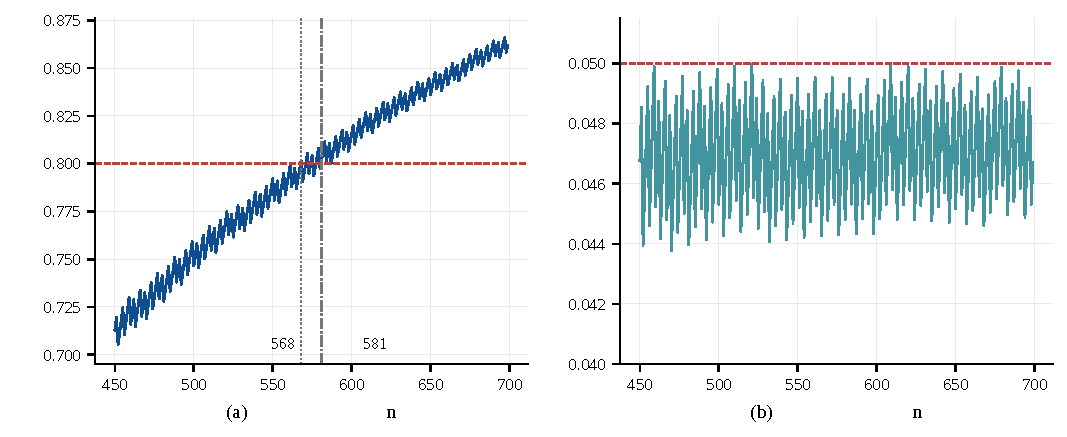
\includegraphics[width=0.95\linewidth]{figures/fig_power_sawtooth.pdf}\caption{精确增长检验的功效与实际水平随上一代感染者数 $n$ 的锯齿变化（$k=0.35$，$\delta=0.30$，$\rho=0.25$，$\alpha=0.05$）。左图为精确功效，红虚线为 0.8，两条竖线分别标出首次达到 0.8 的 $n=568$ 与此后稳定不低于 0.8 的 $n=581$；右图为实际检验水平，始终不超过 0.05 并随临界值跳升锯齿波动。}\label{fig:pb-power}\end{figure}

由于功效非单调，“首次达到 0.8 的 $n$”与“此后恒不低于 0.8 的 $n$”是两个不同的量。表~\ref{tab:pb-power} 列出论文图 2 的五组配置，稳定样本量比首次样本量多 1.4\%–3.0\%。

\begin{table}[!tbp]\centering\small\caption{论文图 2 五组配置下首次与稳定达到 80\% 功效的样本量（$\rho=0.25$，$\alpha=0.05$）}\label{tab:pb-power}
\begin{tabular}{L{1.6cm}L{1.6cm}L{2.4cm}L{2.4cm}L{2.0cm}L{3.2cm}}
\toprule
$k$ & $\delta$ & 首次 $n$（$m=\rho n$） & 稳定 $n$（$m=\rho n$） & 增幅 & 首次之后跌回 0.8 以下的 $n$ 个数 \\
\midrule
0.35 & 0.15 & 2071（517.75） & 2107（526.75） & 1.7\% & 19 \\
0.35 & 0.30 & 568（142.00） & 581（145.25） & 2.3\% & 7 \\
0.35 & 0.50 & 229（57.25） & 235（58.75） & 2.6\% & 2 \\
1.0 & 0.25 & 568（142.00） & 585（146.25） & 3.0\% & 9 \\
0.1 & 0.25 & 1660（415.00） & 1684（421.00） & 1.4\% & 10 \\
\bottomrule
\end{tabular}
\end{table}

Wald 检验的精确水平可以按式~\eqref{eq:pb-wald} 手算。取 $m=5$（$n=20$）、$k=0.1$：$V_0=1/5+1/2=0.7$，$\sqrt{V_0}=0.8367$，$z_{0.95}=1.6449$，阈值 $5\times(1+1.6449\times0.8367)=11.88$，取整为 12；$C_t\sim\mathrm{NB}(2,\,0.1/0.35)$ 时 $\Pr(C_t\ge12)=0.0781$，高于名义水平 0.05。

\subsubsection{与仿真和实证的对应}

论文图 2（原文第 353–359 行）检验的就是命题 6。核验结果如下。
\begin{itemize}
\item 符号核验确认式~\eqref{eq:pb-lr} 的对数斜率与 $1-p^*$ 的导数；在 200 组随机 $(n,k,R<R')$ 下，似然比在 $j=0,\dots,499$ 上严格递增，没有违例。$n=100$、$k=0.35$ 时尾概率在 $R\in[0.3,1]$ 上单调，最大值 0.0488 在 $R=1$ 处取得。
\item 在 $k\in\{0.1,0.35,1\}$、$n\le3000$ 的网格上，精确检验的实际水平最大 0.05000、最小 0.01696，没有恰好等于 0.05 的点；$c_\alpha(n)$ 关于 $n$ 单调不减。
\item 图 2(b)(c) 报告的五个“首次达到 80\% 功效”的 $n$（2071/568/229/568/1660）全部被精确复现；图 2(c) 所说“近 3 倍”的样本需求放大实为 2.92 倍。
\item 图 2(a) 的 Wald 检验经验水平可以由式~\eqref{eq:pb-wald} 精确计算：$m=5$、$k=0.1$ 时精确值 0.0781，论文 30000 次模拟的 0.081 落在模拟误差 $\pm2\sigma$（$\pm0.0031$）带内，$2\times10^5$ 次复核得 0.0789；$k=1$ 时精确值 0.0493 与 0.0691，与论文的 0.0495 与 0.0691 一致。在 $k\le0.35$、$m<40$ 的 14 个网格点上精确水平全部高于 0.05，论文“系统性过检”的结论成立。
\end{itemize}

\subsubsection{原文表述的问题}

\begin{itemize}
\item 第 340 行称非随机化检验的实际水平“严格低于名义水平 $\alpha$”，一般陈述中应改为“不超过 $\alpha$”；第 323 行“严格控制在 $\alpha$ 以内”的表述可以保留。
\item 正文若使用“最优”一词，应写明非随机化检验只在它的实际水平下一致最优；若需要恰好水平 $\alpha$，可改用第 6 步的随机化检验。
\item 以上结论都在 $k$ 已知时成立；实际应用中以估计值 $\hat k$ 代入时水平不再有精确保证，论文的局限性部分应补充这一点。
\item 图 2 只报告首次达到 80\% 功效的 $n$，建议同时报告表~\ref{tab:pb-power} 的稳定样本量；第 364 行的 Wald 水平建议改报式~\eqref{eq:pb-wald} 的精确值。
\end{itemize}

\subsection{更新过程仿真中的恒等式}

\subsubsection{原式与参数含义}

论文在时间序列更新过程中评价两类误差，所用的恒等式与分解是命题 5 在仿真中的落地形式。预测时刻已知的历史报告加权和定义如下：
\begin{equation*}
D_t \triangleq \sum_{s=1}^S w_s C_{t+1-s}.
\tag{原文式 26}
\end{equation*}
事后代理增长统计量由原文第 379 行定义如下：
\begin{equation*}
G_{t+1} \triangleq C_{t+1}/D_t
\tag*{原文第 379 行}
\end{equation*}
事前单步预测由原文第 380 行定义如下：
\begin{equation*}
\widehat{C}_{t+1 \mid t} \triangleq \bar{R} D_t
\tag*{原文第 380 行}
\end{equation*}
两者的误差由下面的恒等式联系起来：
\begin{equation*}
\operatorname{RelMSE}(m) \triangleq \mathbb{E}\left[\left(\frac{C_{t+1} - \widehat{C}_{t+1 \mid t}}{\widehat{C}_{t+1 \mid t}}\right)^2 \;\middle|\; D_t > 0\right] = \frac{1}{\bar{R}^2}\mathbb{E}\left[(G_{t+1} - \bar{R})^2 \;\middle|\; D_t > 0\right].
\tag{原文式 27}
\end{equation*}
条件预测矩由原文第 387 行定义如下：
\begin{equation*}
\mu_{t+1 \mid t} \triangleq \mathbb{E}[C_{t+1} \mid \mathcal{F}_t^C]
\tag*{原文第 387 行}
\end{equation*}
\begin{equation*}
\sigma_{t+1 \mid t}^2 \triangleq \operatorname{Var}(C_{t+1} \mid \mathcal{F}_t^C)
\tag*{原文第 387 行}
\end{equation*}
活跃周上的条件分解如下：
\begin{equation*}
\mathbb{E}\left[(G_{t+1} - \bar{R})^2 \;\middle|\; D_t > 0\right] = \mathbb{E}\left[\frac{\sigma_{t+1 \mid t}^2}{D_t^2} + \left(\frac{\mu_{t+1 \mid t}}{D_t} - \bar{R}\right)^2 \;\middle|\; D_t > 0\right].
\tag{原文式 28}
\end{equation*}
参照曲线 $V(m)=v_R+A/m$ 在规模翻倍时的相对降幅如下：
\begin{equation*}
\frac{V(m) - V(2m)}{V(m)} = \frac{1}{2(1 + m/m_\times)}.
\tag{原文式 29}
\end{equation*}

各式中出现的参数含义如下。
\begin{itemize}
\item $D_t\ge0$ 是用报告病例按世代间隔权重 $w_s$ 加权得到的历史规模，它关于 $\mathcal F_t^C$ 可测；给定真实感染历史时 $\mathbb E[D_t\mid I]=\rho\Lambda_{t+1}$，所以 $D_t$ 是感染压力的一个带二项噪声的代理。
\item $G_{t+1}$ 是事后代理增长统计量，只在 $D_t>0$ 的活跃周有定义。
\item $\widehat C_{t+1\mid t}$ 是以已知基础水平 $\bar R$ 乘历史规模得到的事前预测；$\operatorname{RelMSE}(m)$ 是活跃周上的相对均方预测误差，$m$ 是每条仿真轨迹的初始期望报告规模。
\item $\mu_{t+1\mid t}$ 与 $\sigma^2_{t+1\mid t}$ 是给定报告历史时下一期报告数的条件均值与条件方差，后者就是命题 5 中原文式 22 的左端。
\item $V(m)=v_R+A/m$ 是命题 2 的单代参照曲线，$m_\times=A/v_R$ 是交叉点；仿真取图 1 参数，$m_\times=53.08$，$\bar R=1.15$，$\bar R^2=1.3225$。
\end{itemize}

\subsubsection{逐步推导}

原文式 27 只用到代数恒等变形，推导分三步。
\begin{enumerate}
\item 在 $D_t>0$ 的事件上代入 $\widehat C_{t+1\mid t}=\bar RD_t$，分子分母同除以 $D_t$，得 $(C_{t+1}-\bar RD_t)/(\bar RD_t)=(G_{t+1}-\bar R)/\bar R$。
\item 两边平方，得到逐观测成立的等式，左端是相对预测误差的平方，右端是 $(G_{t+1}-\bar R)^2/\bar R^2$。
\item 由条件期望的线性性，在同一事件 $\{D_t>0\}$ 上取条件期望，并把常数 $1/\bar R^2$ 提到期望外，即得原文式 27。由于等式逐观测成立，它对同一活跃周子集上的样本平均同样成立，两类误差的翻倍降幅中常数 $1/\bar R^2$ 相消，所以两者的经验降幅完全相同。
\end{enumerate}

原文式 28 的推导要用到“提出已知量”与塔式性质，分五步。
\begin{enumerate}
\item 以 $\mu=\mu_{t+1\mid t}$ 为中心作加减拆分，得 $G_{t+1}-\bar R=(C_{t+1}-\mu)/D_t+(\mu/D_t-\bar R)$。第一项是围绕条件均值的波动，第二项是用报告历史代理感染压力造成的偏差。
\item 由完全平方公式展开，平方项分成波动平方 $(C_{t+1}-\mu)^2/D_t^2$、交叉项 $2(C_{t+1}-\mu)(\mu/D_t-\bar R)/D_t$ 与偏差平方 $(\mu/D_t-\bar R)^2$ 三部分。
\item 由于 $D_t$ 由 $C_t,\dots,C_{t+1-S}$ 构成，它关于 $\mathcal F_t^C$ 可测，$\mu$ 也关于 $\mathcal F_t^C$ 可测。由条件期望“提出已知量”的性质，波动平方的条件期望为 $\sigma^2_{t+1\mid t}/D_t^2$，偏差平方原样保留，交叉项的条件期望含因子 $\mathbb E[C_{t+1}-\mu\mid\mathcal F_t^C]=0$，因而为零。
\item 于是在 $\{D_t>0\}$ 上有 $\mathbb E[(G_{t+1}-\bar R)^2\mid\mathcal F_t^C]=\sigma^2_{t+1\mid t}/D_t^2+(\mu_{t+1\mid t}/D_t-\bar R)^2$。
\item 事件 $\{D_t>0\}$ 属于 $\mathcal F_t^C$，由塔式性质，对第 4 步两端再取以该事件为条件的期望，即得原文式 28。
\end{enumerate}

原文式 29 的推导分三步。
\begin{enumerate}
\item 由 $V(m)=v_R+A/m$，环境项在差分中相消，分子为 $V(m)-V(2m)=A/m-A/(2m)=A/(2m)$。
\item 除以 $V(m)$ 并把分子分母同乘 $m$，得 $A/[2(v_Rm+A)]$。
\item 分子分母同除以 $A$，并代入 $m_\times=A/v_R$，即得原文式 29。这个降幅等于规模项在总方差中所占份额的一半，上限 50\% 只在 $m\to0$ 时取到。
\end{enumerate}

最后说明原文式 28 推不出“经验误差始终不低于单代下界”，理由分三步。
\begin{enumerate}
\item 原文式 28 中偏差项非负，由期望的单调性只能得到 $\mathbb E[(G_{t+1}-\bar R)^2\mid D_t>0]\ge\mathbb E[\sigma^2_{t+1\mid t}/D_t^2\mid D_t>0]$。
\item 若要进一步得到不低于 $v_R+A/m$，还需要右端不低于 $v_R+A/m$。式~\eqref{eq:pb-expand} 给出的是 $\sigma^2_{t+1\mid t}$ 除以 $(\rho E_\Lambda)^2$ 后的展开，原文式 28 除的却是报告历史 $D_t^2$；$D_t/(\rho E_\Lambda)$ 是随机比值，增长期的 $\mu/D_t$ 也会偏离 $\bar R$，所以两者的大小关系方向不定。
\item 参照曲线中的 $m$ 是初始规模，增长期评价周的实际规模远大于初始值，横轴口径不同也会改变比较结果。因此“始终不低于单代下界”只能作为特定口径下的经验观察，没有定理的地位。
\end{enumerate}

\subsubsection{直觉与数值例}

原文式 27 说明事前预测误差与事后增长统计量误差是同一个量的两种写法。原文式 28 把它拆成两块：随机分母使条件方差按 $1/D_t^2$ 重新加权，偏差项则反映用报告历史代替真实感染压力的系统误差。

翻倍降幅按原文式 29 计算，图 1 参数下 $m_\times=53.08$。$m=10$ 时降幅为 42.1\%，$m=m_\times$ 时为 25.0\%，$m=200$ 时为 10.5\%，首点 $m=6$ 时为 44.9\%。

小规模端的数值都可以由参照曲线逐项复算，表~\ref{tab:pb-small} 汇总了 $m=6$ 与 $m=12$ 两组的计算过程。$m=6$ 时经验相对误差是参照值的 1.82 倍；$m=12$ 时经验值 0.190 已低于参照值 0.217；首点 $m=6\to12$ 的经验翻倍降幅 73.5\% 远高于原文式 29 给出的 44.9\%。

\begin{table}[!tbp]\centering\small\caption{更新过程仿真小规模端数值的复算（图 1 参数）}\label{tab:pb-small}
\begin{tabular}{L{4.6cm}L{5.4cm}L{2.4cm}}
\toprule
量 & 计算 & 结果 \\
\midrule
$m=6$ 参照值 $v_R+A/6$ & $0.04+2.12321/6$ & 0.394 \\
$m=6$ 参照相对误差 & $0.39387/1.3225$ & 0.298 \\
$m=6$ 经验相对误差 & 论文报告值 & 0.543 \\
$m=6$ 经验与参照之比 & $0.543/0.298$ & 1.82 \\
$m=12$ 参照值 $v_R+A/12$ & $0.04+2.12321/12$ & 0.217 \\
$m=12$ 经验值 & 论文报告值 & 0.190 \\
环境底板 $v_R/\bar R^2$ & $0.04/1.3225$ & 0.0302 \\
首点经验翻倍降幅 & $(0.543\times1.3225-0.190)/(0.543\times1.3225)$ & 73.5\% \\
\bottomrule
\end{tabular}
\end{table}

\subsubsection{与仿真和实证的对应}

这一组恒等式对应论文图 3 以及第 393、399、405、406、409 行的文字，核验结果如下。
\begin{itemize}
\item 原文式 27 的逐观测恒等与原文式 28 的条件分解经符号核验成立；在 $m=6$ 到 200 的各规模组上，分解两端的蒙特卡洛估计彼此一致。
\item 表~\ref{tab:pb-small} 的全部数值以及论文报告的剔除率（$m=6$ 组 0.077\%，$m=12$ 组 0.026\%）均被复现；翻倍降幅 42.1\%、25.0\%、10.5\% 与原文式 29 的代入结果一致。
\item 第 393 行的横轴口径数值可以复现到相近范围。按初始 $m$，$m\ge25$ 段经验与参照之比在论文中为 0.75–0.98，本讲义重算为 0.77–0.92；按实现规模分箱，论文为 1.01–1.17，重算为 1.03–1.12；评价周实际规模中位数与初始 $m$ 之比，论文为 1.7–2.4 倍，重算为 1.82–2.36 倍。
\end{itemize}
按初始规模的比值低于 1，说明参照曲线在这一口径下高于经验误差；只有按实现规模分箱时比值才高于 1。第~\ref{sec:empirical} 节的实证分母同样由报告病例构造，随机分母对斜率的放大与这里 $1/D_t^2$ 的重新加权属于同一机制。

\subsubsection{原文表述的问题}

\begin{itemize}
\item 第 393 行与第 406 行称更新过程经验误差“始终不低于单代静态下界”，并把它与原文式 28 联系起来。由上文推导的最后三步，原文式 28 只保证偏差项非负，推不出不低于 $v_R+A/m$；按初始规模的比值 0.75–0.98 本身就低于 1。建议改为“按实现规模分箱时，本仿真中经验误差不低于参照曲线（1.01–1.17 倍），方向与非负偏差项一致，但这不构成一般性下界”。
\item 第 375 行的 $\max(1,I)$ 截断改变了小规模端的数据生成过程，论文说明了偏差方向，但没有报告各规模组的触发频率，建议补充，尤其是 $m=6$ 组。
\item 首点经验降幅 73.5\% 高于解析值 44.9\%，正文可以补一句原因：小规模端的偏差项与随机分母的贡献随规模迅速衰减，降幅因此叠加了参照曲线之外的部分。
\end{itemize}
